\documentclass[11pt,a4paper]{article}
\usepackage[T1]{fontenc}
\usepackage[margin=2.3cm]{geometry}
\usepackage{amsmath,amssymb}
\usepackage{graphicx}
\usepackage[dvipsnames]{xcolor}
\usepackage{enumitem}
\usepackage[colorlinks=true,linkcolor=blue,urlcolor=blue]{hyperref}
\setlength{\parskip}{0.6em}
\setlength{\parindent}{0pt}
\begin{document}

\begin{center}{\LARGE\bfseries opensql}\\[0.4em]{\large Ask a database a question, then design its tables, in three sessions.}\\[0.2em]\small PAN IIT OSS explainer \textbullet{} secondary school to diploma / undergraduate (levels 3-5)\end{center}

\section*{Why this exists}
Almost every app keeps its data in tables and asks questions with SQL. This explainer shows what a table is, how a query is answered, why tables are split, and why indexes and transactions matter, using only Python's built-in sqlite3, so you can run everything yourself.

\section*{The end goal}
Query a small database and design its tables. The end goal is to query a small database and design its tables: choose columns and keys, split data so each fact is stored once, write filters, joins and summaries, and know what makes a query fast, safe and right. The same ideas carry over to PostgreSQL, MySQL and the databases behind most websites.

\section*{How the three sessions build up}
\begin{enumerate}[nosep]
\item \textbf{Session 1: A table is a grid, a query asks it a question} (Level 1, conceptual interactive model, 60 min).
\item \textbf{Session 2: Ask precise questions, and store every fact once} (Level 2, mathematical engineering model, 80 min).
\item \textbf{Session 3: How fast, how safe, how right} (Level 3, simulation and validation, 90 min).
\end{enumerate}

\section{Session 1: A table is a grid, a query asks it a question}

\subsection*{A. Real-world problem}
A school keeps marks for hundreds of students. The teacher asks 'who scored at least 60?' or 'who is in grade 9 or above and scored at least 70?'. Nobody wants to read every row. A database keeps the rows in a table, and a query asks the question for us. How do we write the question so a computer can answer it, and how do we know the answer is right? (All names and marks here are synthetic.)

\subsection*{B. Concept and theory}
A table is a grid. Each row is one record (one student) and each column is one fact (name, grade, marks) stored for every record. A query is a question asked of the table. In SQL, SELECT says which columns to show, FROM says which table, and WHERE keeps only the rows for which a condition is true; the other rows are dropped. A query only reads: it never changes the table. Conditions use comparisons (\textgreater{}=, \textgreater{}, =) and can be joined with AND (both must hold) or OR (either holds). We always check a query against an independent computation, here a Python list comprehension and a numpy mask.

\begin{itemize}[nosep]
\item m: marks cut-off in the condition marks \textgreater{}= m (marks)
\item g: grade cut-off in the condition grade \textgreater{}= g (grade)
\item n\_kept: number of rows that pass the filter (rows)
\item N: number of rows in the table (12) (rows)
\end{itemize}

\begin{equation*}
n_{\text{kept}}=\left|\{\,r : \text{marks}(r)\ge m \ \wedge\ \text{grade}(r)\ge g\,\}\right|
\end{equation*}

\begin{equation*}
\text{percent kept}=100\,\frac{n_{\text{kept}}}{N}
\end{equation*}

\begin{center}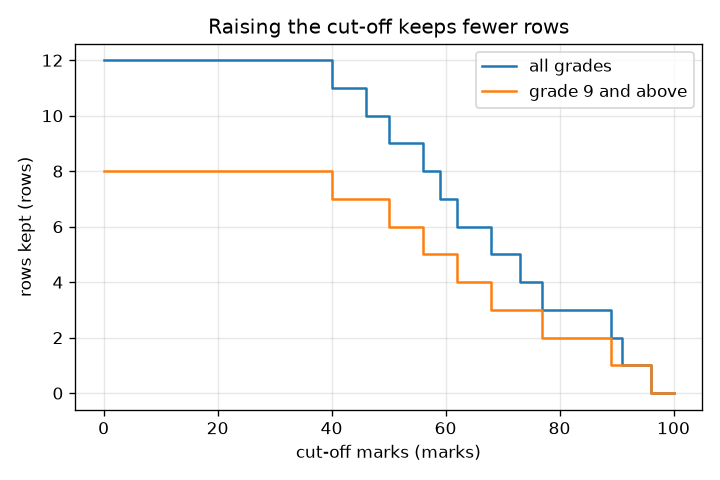
\includegraphics[width=0.85\linewidth]{figures/s01_rows_vs_cutoff.png}\\\small Rows kept against the cut-off: a staircase that only falls as the cut-off rises.\end{center}

\subsection*{E. Worked example}
Using the 12-row table, which students are in grade 9 or above and scored at least 70? How many rows are in grade 9 or above to begin with?
\begin{enumerate}[nosep]
\item Rows with grade \textgreater{}= 9: Chitra (9), Dev (9), Farid (10), Gita (10), Hari (9), Indu (10), Kavya (9), Lalit (10). That is 8 rows.
\item Of those, marks \textgreater{}= 70: Chitra 88 yes, Dev 61 no, Farid 55 no, Gita 67 no, Hari 39 no, Indu 95 yes, Kavya 76 yes, Lalit 49 no.
\item Three rows pass: Chitra, Indu, Kavya.
\item SQL: SELECT name FROM students WHERE grade \textgreater{}= 9 AND marks \textgreater{}= 70 ORDER BY id; gives the same three names.
\end{enumerate}
\textbf{Answer.} Chitra, Indu and Kavya (3 rows), chosen from the 8 rows with grade 9 or above.

\subsection*{F. Questions}
\begin{enumerate}[nosep]
\item \textbf{Conceptual.} Does running a SELECT query change the table? Why does the order of rows in an answer need an ORDER BY?
\item \textbf{Numerical.} How many rows have grade 10 and marks of at least 50? What percentage of the whole table is that?
\item \textbf{Graph and simulation interpretation.} On the staircase graph for all grades, how many rows are kept at a cut-off of 90, and what is the first whole-number cut-off that keeps 0 rows?
\item \textbf{Design and optimisation challenge.} Design: a scholarship interview should include exactly the top 3 students out of 12 (25 percent) by marks. Choose a cut-off for 'marks \textgreater{}= cut-off'. Which cut-offs work, and which one would you pick?
\end{enumerate}

\section{Session 2: Ask precise questions, and store every fact once}

\subsection*{A. Real-world problem}
A school has 40 students and three subjects: 120 marks. The head teacher wants the best five Science scores, the average per subject, and the students whose average is at least 75. Then a shop owner shows a spreadsheet where every order repeats the customer's city, and asks why one customer ended up in two cities after an edit. Finally a librarian asks for the list of overdue books. How do we ask precisely, and how do we store data so these problems cannot happen?

\subsection*{B. Concept and theory}
Aggregate functions collapse many rows into one number: COUNT counts rows, SUM adds, AVG is SUM divided by COUNT, MIN and MAX pick the extremes. GROUP BY makes one answer row per group. WHERE filters rows before grouping; HAVING filters groups after it. ORDER BY sorts and LIMIT keeps the first few. A primary key identifies each row once. A foreign key is a column whose values must exist in another table's primary key; the database rejects a row that points nowhere (when foreign keys are switched on). One big table that repeats facts (a customer's city on every order) allows anomalies: an update done on only some rows leaves contradictions, a new customer cannot be recorded without an order, and deleting the last order deletes the only record of the customer. Normalisation cures this. 1NF: every cell holds one value. 2NF: every non-key column depends on the whole key. 3NF: no non-key column depends on another non-key column. In the order table, city depends on customer and price depends on item, so we give customers and items their own tables and keep only their keys in orders.

\begin{itemize}[nosep]
\item n: number of orders stored (orders)
\item k: number of customers (customers)
\item m: number of items on sale (3 here) (items)
\item cells: rows times columns, summed over the tables (cells)
\item AVG: average of a group of numbers = SUM / COUNT (same unit as the data)
\end{itemize}

\begin{equation*}
\text{AVG}=\frac{\text{SUM}}{\text{COUNT}}
\end{equation*}

\begin{equation*}
\text{cells}_{\text{big}}=6n,\qquad \text{cells}_{\text{3NF}}=4n+3k+3m
\end{equation*}

\begin{equation*}
\text{rows to edit when one customer moves}\approx\frac{n}{k}\ \text{(big table)},\quad 1\ \text{(3NF)}
\end{equation*}

\begin{center}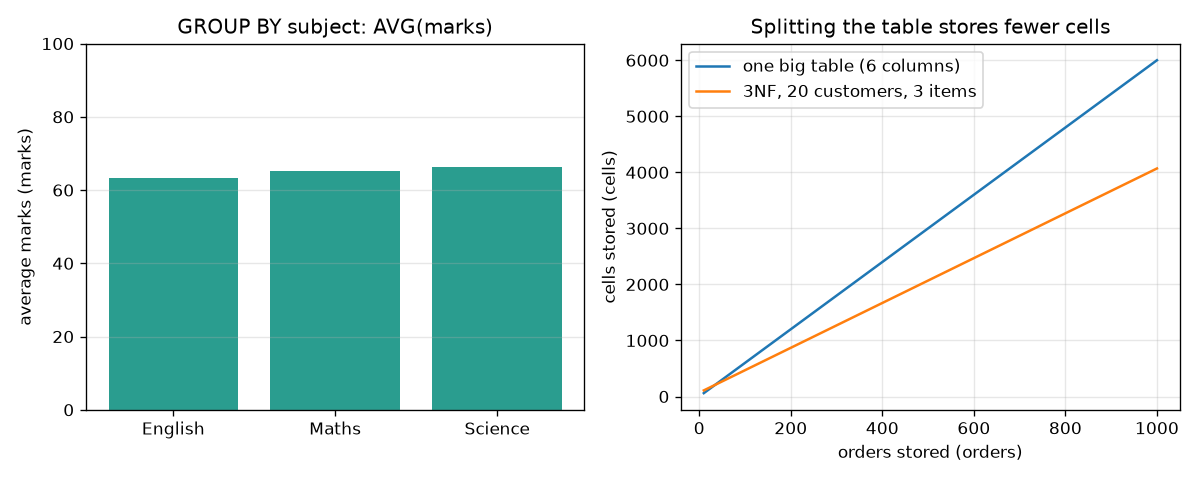
\includegraphics[width=0.85\linewidth]{figures/s02_queries_and_cells.png}\\\small Left: GROUP BY subject, average marks. Right: cells stored by the big table (6n) and by three tables (4n + 3k + 9).\end{center}

\subsection*{E. Worked example}
A six-row table has marks: Maths 70, 90, 80 and Science 60, 50, 85. Use GROUP BY subject to find each subject's sum and average, and use HAVING AVG(marks) \textgreater{} 70 to keep the strong subjects.
\begin{enumerate}[nosep]
\item Maths group: 70 + 90 + 80 = 240; COUNT = 3; AVG = 240 / 3 = 80.
\item Science group: 60 + 50 + 85 = 195; COUNT = 3; AVG = 195 / 3 = 65.
\item HAVING AVG \textgreater{} 70 keeps groups whose average is above 70: Maths (80) stays, Science (65) goes.
\item HAVING is strict, so AVG \textgreater{} 80 would keep nothing, and AVG \textgreater{} 60 would keep both.
\end{enumerate}
\textbf{Answer.} Maths: sum 240, average 80, kept. Science: sum 195, average 65, dropped.

\subsection*{F. Questions}
\begin{enumerate}[nosep]
\item \textbf{Conceptual.} Why can you not write WHERE AVG(marks) \textgreater{}= 75 to find students whose average is at least 75? What do you write instead?
\item \textbf{Numerical.} A shop has 500 orders and 10 customers and sells 3 items. How many cells does the big table store, how many do the three tables store, and what percentage is that?
\item \textbf{Graph and simulation interpretation.} In the line chart with k = 20 customers and 3 items, between which two numbers of orders do the lines cross? What does that tell a designer?
\item \textbf{Design and optimisation challenge.} Design: a library lends books to members. Design the tables with keys, and write the query that lists loans that are overdue today (still out and due before today), with the member name, the title and the days late.
\end{enumerate}

\section{Session 3: How fast, how safe, how right}

\subsection*{A. Real-world problem}
A shop database holds 200,000 rows. One query finds a customer's orders in a blink and another makes the page hang. A transfer between two accounts must never lose money, even if the power fails half-way. And a search box must never let a visitor's text become part of the program. What do we measure to know a query is fast, what guarantees a transfer, and what makes a query safe?

\subsection*{B. Concept and theory}
A JOIN pairs rows of two tables whose key columns match; it is a nested loop with a condition. An inner join keeps only matched pairs, a left join also keeps unmatched rows of the left table, filling the other side with NULL. Without an index the database must scan every row to find a match, so the cost grows in proportion to the number of rows n. An index is a sorted structure (a B-tree) kept beside the table. Each B-tree node holds up to B keys, so each step down divides the remaining rows by about B and the number of levels d is the smallest d with B\textasciicircum{}d \textgreater{}= n. A transaction groups statements so they all happen (COMMIT) or none do (ROLLBACK); a transfer therefore conserves the total money. A query built by gluing text into SQL lets the text change the query's meaning (SQL injection); parameters (?) keep data and SQL separate. Timings depend on the computer and are illustrative; plans, step counts and results are exact.

\begin{itemize}[nosep]
\item n: number of rows in the table (rows)
\item B: keys per B-tree node (keys)
\item d: levels of the B-tree = steps to find one row (levels)
\item steps: virtual-machine instructions run by SQLite for one query (steps)
\item T: total money in all accounts (rupees)
\end{itemize}

\begin{equation*}
d=\min\{\,d\ge 1 : B^{d}\ge n\,\}\approx\left\lceil \frac{\log n}{\log B}\right\rceil
\end{equation*}

\begin{equation*}
\text{binary search comparisons}=\lceil \log_2 n\rceil
\end{equation*}

\begin{equation*}
\text{cost}_{\text{scan}}\propto n,\qquad \text{cost}_{\text{index}}\propto \log_B n
\end{equation*}

\begin{equation*}
T_{\text{before}}=T_{\text{after}}\quad\text{for every committed or rolled-back transfer}
\end{equation*}

\begin{center}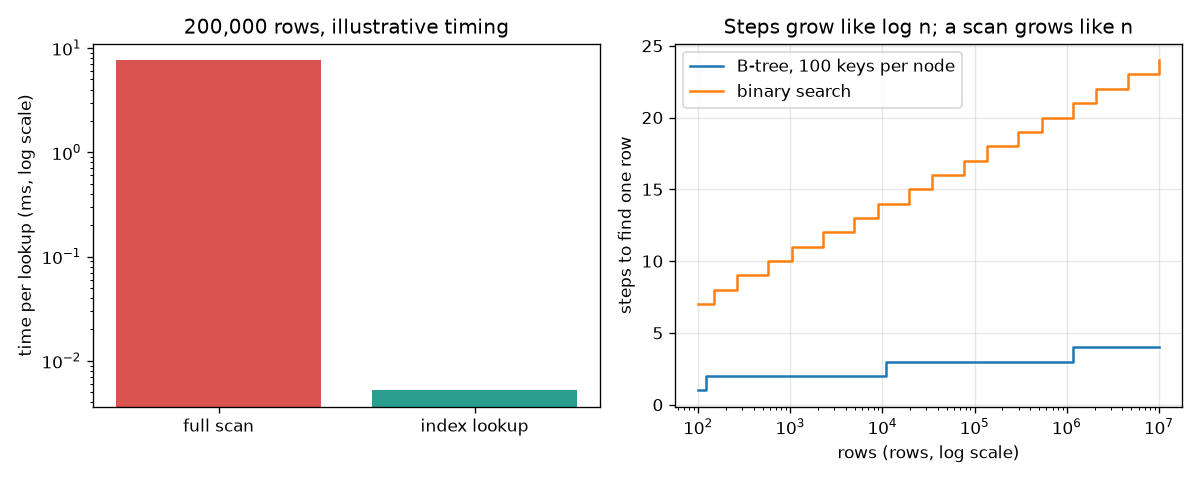
\includegraphics[width=0.85\linewidth]{figures/s03_scan_vs_index.png}\\\small Left: time per lookup on 200,000 rows, scan versus index (log scale, illustrative). Right: steps to find one row, B-tree versus binary search.\end{center}

\subsection*{E. Worked example}
A table has 1,000,000 rows and each B-tree node holds 100 keys. How many levels does an index lookup need, how many comparisons does binary search need, and how many rows might a scan read?
\begin{enumerate}[nosep]
\item Levels: find the smallest d with 100\textasciicircum{}d \textgreater{}= 1,000,000. 100\textasciicircum{}1 = 100, 100\textasciicircum{}2 = 10,000, 100\textasciicircum{}3 = 1,000,000. So d = 3.
\item Binary search halves the range each time: 2\textasciicircum{}19 = 524,288 \textless{} 1,000,000 \textless{}= 2\textasciicircum{}20 = 1,048,576, so 20 comparisons.
\item A scan reads the rows one by one: up to 1,000,000.
\item One more row (1,000,001) already needs 4 levels, because 100\textasciicircum{}3 is exactly 1,000,000.
\end{enumerate}
\textbf{Answer.} 3 levels for the B-tree, 20 comparisons for binary search, up to 1,000,000 rows for a scan.

\subsection*{F. Questions}
\begin{enumerate}[nosep]
\item \textbf{Conceptual.} Why does a parameterised query (WHERE name = ?) stop SQL injection, while gluing the name into the string does not?
\item \textbf{Numerical.} A table has 50,000,000 rows. How many levels does a B-tree with 200 keys per node need, and how many comparisons does binary search need?
\item \textbf{Graph and simulation interpretation.} On the right-hand chart, how many levels does the B-tree need at 1,000,000 rows, and at 1,000,001 rows? Why is the curve a staircase?
\item \textbf{Design and optimisation challenge.} Design: the 200,000-row orders table gets 50 lookups per second by customer and 1 new order per second. Should cust\_id be indexed? Name one benefit, one cost and one more place you would add an index.
\end{enumerate}

\section{Real-world mini-project}
\textbf{Schema and three reports for a small canteen.} A school canteen sells six items to eight regular customers. Session 3 provides the synthetic data (\texttt{CANTEEN\_ITEMS}, \texttt{CANTEEN\_CUSTOMERS}, \texttt{canteen\_sales()}) and a plain Python reference (\texttt{canteen\_reference()}). Create the three tables with primary and foreign keys (items, customers, sales), load the data, and write the SQL for three reports: (1) revenue per item, highest first, (2) customers who spent at least 200 rupees in total, highest first, (3) items that were never sold. Revenue is quantity times price.

\section{The path ahead}
\begin{enumerate}[nosep]
\item \textbf{Session 4: Composite and covering indexes.} A query tuned with the right composite index, with before-and-after plans.
\item \textbf{Session 5: Window functions and running totals.} A canteen report with a running revenue column per customer.
\item \textbf{Session 6: Messy spreadsheet to third normal form.} A script that loads a 1,000-row flat order file and builds customers, items and orders tables.
\item \textbf{Session 7: Concurrency and the write-ahead log.} Several threads transferring money at the same time against one file database.
\item \textbf{Session 8: A tiny B-tree and the query visualiser.} Your own B-tree with insert and search, drawn step by step, plus a visualiser like the Target.
\end{enumerate}

\section{Answers and hints}

\subsection*{Session 1}
\begin{enumerate}[nosep]
\item \textbf{Conceptual.} Hint: Think about what 'read' and 'write' mean, and about whether a table promises any order. Solution: No: SELECT only reads. Changing data needs INSERT, UPDATE or DELETE. A table is a set of rows and does not promise to return them in any particular order, so if the order matters (for example highest marks first) you must say so with ORDER BY.
\item \textbf{Numerical.} Hint: List the four grade 10 rows first, then apply marks \textgreater{}= 50. Solution: Grade 10 rows: Farid 55, Gita 67, Indu 95, Lalit 49. Marks \textgreater{}= 50 keeps Farid, Gita and Indu: 3 rows. Percentage = 100 * 3 / 12 = 25 percent. Sanity check: 3 is no more than the 4 grade 10 rows.
\item \textbf{Graph and simulation interpretation.} Hint: Marks of 90 or more: look for the largest marks in the table. Solution: Marks \textgreater{}= 90: Esha 90 and Indu 95, so 2 rows. The largest mark is 95, so a cut-off of 95 keeps 1 row and 96 is the first cut-off that keeps 0 rows. The staircase drops to 0 just after 95.
\item \textbf{Design and optimisation challenge.} Hint: The top marks are 95, 90, 88, 76. Where must the cut-off lie to keep the first three but not the fourth? Solution: The cut-off must be above 76 (otherwise Kavya is kept) and at most 88 (otherwise Chitra is lost). So whole-number cut-offs 77 to 88 keep exactly 3 rows. A cut-off of 80 is a sensible choice because it sits in the middle of the gap between 76 and 88 and is easy to explain. Trade-off: with real data, ties at the boundary would make the number of rows jump.
\end{enumerate}

\subsection*{Session 2}
\begin{enumerate}[nosep]
\item \textbf{Conceptual.} Hint: When is WHERE applied: before or after the rows are grouped? Solution: WHERE filters individual rows before any grouping, so the average does not exist yet at that point. The average belongs to a group, so the condition goes after the grouping, in HAVING: SELECT student\_id, AVG(marks) FROM scores GROUP BY student\_id HAVING AVG(marks) \textgreater{}= 75. In the synthetic school data this returns 8 students.
\item \textbf{Numerical.} Hint: Use 6n for the big table and 4n + 3k + 3m for the three tables. Solution: Big table: 6 * 500 = 3000 cells. Three tables: 4 * 500 + 3 * 10 + 3 * 3 = 2000 + 30 + 9 = 2039 cells. Percentage = 100 * 2039 / 3000 = 68.0 percent. Sanity check: the orders table has 4 of the 6 columns, so the result must be close to 4/6 = 67 percent, and it is. The real gain is not space but safety from anomalies.
\item \textbf{Graph and simulation interpretation.} Hint: Solve 6n = 4n + 3k + 9 for n. Solution: 6n = 4n + 69 gives n = 34.5. At 34 orders the big table is smaller (204 against 205 cells); at 35 orders the three tables are smaller (209 against 210). So the lines cross between 34 and 35 orders. For tiny data the split costs a little extra, so the reason to normalise is consistency, and the storage saving appears as the data grow.
\item \textbf{Design and optimisation challenge.} Hint: A member borrows many books over time and a book is borrowed by many members over time, so the link needs its own table with two foreign keys. A loan that has not come back has no return date (NULL). Solution: Tables: books(book\_id PK, title), members(member\_id PK, name), loans(loan\_id PK, book\_id FK to books, member\_id FK to members, loaned\_on, due\_on, returned\_on, where returned\_on is NULL while the book is out). Query: SELECT l.loan\_id, m.name, b.title, julianday(today) - julianday(l.due\_on) AS days\_late FROM loans l JOIN books b ON b.book\_id = l.book\_id JOIN members m ON m.member\_id = l.member\_id WHERE l.returned\_on IS NULL AND l.due\_on \textless{} today. In the sample data with today = 2026-03-10 two loans are overdue: Anita's Malgudi Days (4 days) and Dinesh's Godan (25 days). A loan due today is not yet overdue, and a book returned late is not currently overdue.
\end{enumerate}

\subsection*{Session 3}
\begin{enumerate}[nosep]
\item \textbf{Conceptual.} Hint: Ask who decides where the SQL ends and the data begins. Solution: When text is glued into the SQL string, the database parses the whole string, so quote marks and keywords inside the text become part of the program: the input x' OR '1'='1 turns the condition into one that is always true and returns all 3 users. With a parameter, the SQL is parsed first with a placeholder and the value is supplied afterwards as pure data, so it can only ever be compared with the name column and returns 0 rows. The same fix also makes names such as O'Brien work.
\item \textbf{Numerical.} Hint: Find the smallest d with 200\textasciicircum{}d \textgreater{}= 50,000,000 and the smallest b with 2\textasciicircum{}b \textgreater{}= 50,000,000. Solution: 200\textasciicircum{}3 = 8,000,000 \textless{} 50,000,000 and 200\textasciicircum{}4 = 1,600,000,000 \textgreater{}= 50,000,000, so 4 levels. For binary search 2\textasciicircum{}25 = 33,554,432 \textless{} 50,000,000 \textless{}= 2\textasciicircum{}26 = 67,108,864, so 26 comparisons. Sanity check: the tree is about 6 times shallower than binary search because each node splits the range 200 ways instead of 2.
\item \textbf{Graph and simulation interpretation.} Hint: The number of levels is a whole number that changes at powers of 100. Solution: At 1,000,000 rows it needs 3 levels (100\textasciicircum{}3 = 1,000,000). At 1,000,001 it needs 4, because 100\textasciicircum{}3 is no longer enough. You cannot have 3.2 levels, so the depth jumps by one each time the rows pass a power of B: the curve is a staircase with very long flat steps, which is why an index stays fast as a table grows.
\item \textbf{Design and optimisation challenge.} Hint: Compare the cost of a lookup without and with the index, and ask what an insert has to do to keep an index sorted. Solution: Yes. Benefit: each lookup changes from scanning up to 200,000 rows to about 3 levels, which in the lesson is more than 100 times fewer steps. Cost: every insert must also update the sorted index, so writes are a little slower and the index takes extra space; with 1 insert per second against 50 lookups per second this is clearly worth it. Another candidate is the order date, if reports are asked by date range. Rule of thumb: index columns used in WHERE and JOIN conditions of frequent queries, not every column.
\end{enumerate}

\section{How to join}
Read \texttt{CONTRIBUTING.md} in the repository, then pick an issue labelled \texttt{good first issue}. Repository: \url{https://github.com/KrunalPanchal1995/opensql}

\end{document}
